\documentclass[letterpaper,12pt]{article}
\usepackage{tabularx}
\usepackage{amsmath}  
\usepackage{graphicx}
\usepackage[margin=1in,letterpaper]{geometry} 
\usepackage{cite}
\usepackage[final]{hyperref}
\hypersetup{
	colorlinks=true,    
	linkcolor=blue,        
	citecolor=blue,        
	filecolor=magenta,    
	urlcolor=blue         
}

\begin{document}

\title{Report 1}
\author{Agwu Chinedu}
\date{\today}
\maketitle


\section{Task}

Check if usth.edu.vn is up or not with ping (5 times only)
\begin{itemize}
\item Use traceroute tool to find the route from your VPS to
usth.edu.vn
\item How many hops do you have?
\item Try traceroute again, but from your own computer
\item How many hops do you have?
\end{itemize}

\section{Result and Commands}
The command used for traceroute  was:
\begin{itemize}
\item traceroute usth.edu.vn
\end{itemize}
The result was:
\begin{itemize}
\item 30 loops, 60 bytes packet
\end{itemize}
\begin{figure}[ht] 

        \centering 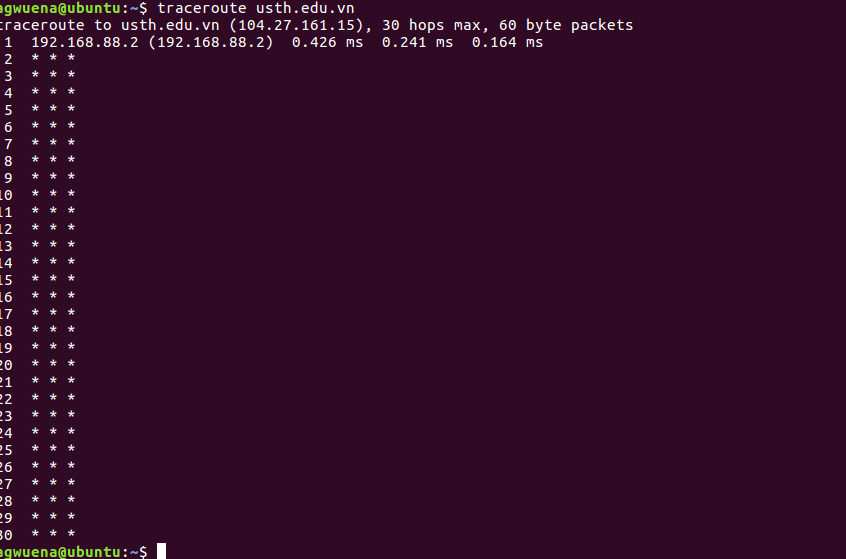
\includegraphics[ height=0.5\columnwidth]{cmd1.png}

        \caption{
                \label{fig:samplesetup}
                 Traceroute Results.
        }
\end{figure}
\begin{figure}[ht] 

        \centering 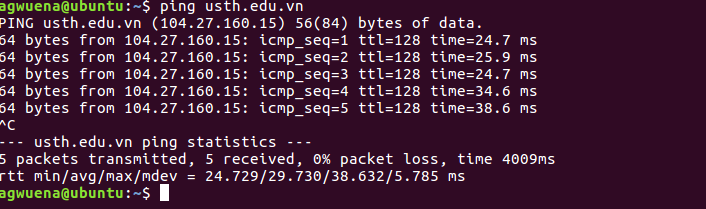
\includegraphics[ width=0.8\columnwidth]{cmd2.png}

        \caption{
                \label{fig:samplesetup}
                 Ping Results.
        }
\end{figure}
The command for ping was:
\begin{itemize}
\item ping usth.edu.vn
\item ctrl + c = interrupt ping
\end{itemize}
The result is also seen in th below figure:
\begin{itemize}
\item 5 packets transmitted with no loss
\item minimum time : 24.729 sec
\item average time : 29.730 sec
\item maximum time : 38.632 sec
\end{itemize}

\end{document}
